\subsection{Helium Embrittlement}
\subsubsection{Helium Production Evaluation}

Helium production within the cladding material during reactor operation is primarily driven by neutron interactions with isotopes present in the cladding alloy. The following reactions contribute significantly to helium generation:
\begin{itemize}
    \item $^{58}$Ni(n,\alpha)$^{55}$Fe (fast neutrons)
    \item $^{59}$Ni(n,\gamma)$^{59}$Ni \rightarrow $^{59}$Ni(n,\alpha)$^{56}$Fe (thermal neutrons)
    \item $^{10}$B(n,\alpha)$^{7}$Li (thermal and fast neutrons)
    \item $^{56}$Fe(n,\alpha)$^{53}$Cr (fast neutrons)
    \item $^{52}$Cr(n,\alpha)$^{49}$Ti (fast neutrons)
\end{itemize}

The time-dependent helium production rate was calculated using Bateman equations, accounting for both isotopic abundance and neutron flux variations over the reactor core height. The primary governing equations for isotopic depletion and helium production are:
\begin{align}
    \frac{dN_{^{58}\text{Ni}}}{dt} &= -\sigma_{^{58}\text{Ni}}^\text{fast} \phi_\text{fast} N_{^{58}\text{Ni}}, \\
    \frac{dN_{^{59}\text{Ni}}}{dt} &= \sigma_{^{58}\text{Ni}}^\text{fast} \phi_\text{fast} N_{^{58}\text{Ni}} - \sigma_{^{59}\text{Ni}}^\text{thermal} \phi_\text{thermal} N_{^{59}\text{Ni}}, \\
    \frac{dN_{^{10}\text{B}}}{dt} &= -\left(\sigma_{^{10}\text{B}}^\text{thermal} \phi_\text{thermal} + \sigma_{^{10}\text{B}}^\text{fast} \phi_\text{fast}\right) N_{^{10}\text{B}},
\end{align}

where $\sigma$ represents the microscopic cross-section for each reaction, $\phi$ is the neutron flux, and $N$ is the atomic concentration of the isotope. The helium production rates are expressed as:
\begin{align}
    \frac{dN_{\text{He}}}{dt} = \sum \text{Contributions from all reactions.}
\end{align}

The cumulative helium production from various isotopes and the total production over time is presented in Figure~\ref{fig:helium_production}, which was obtained by integrating the above equations numerically.

\begin{figure}[H]
    \centering
    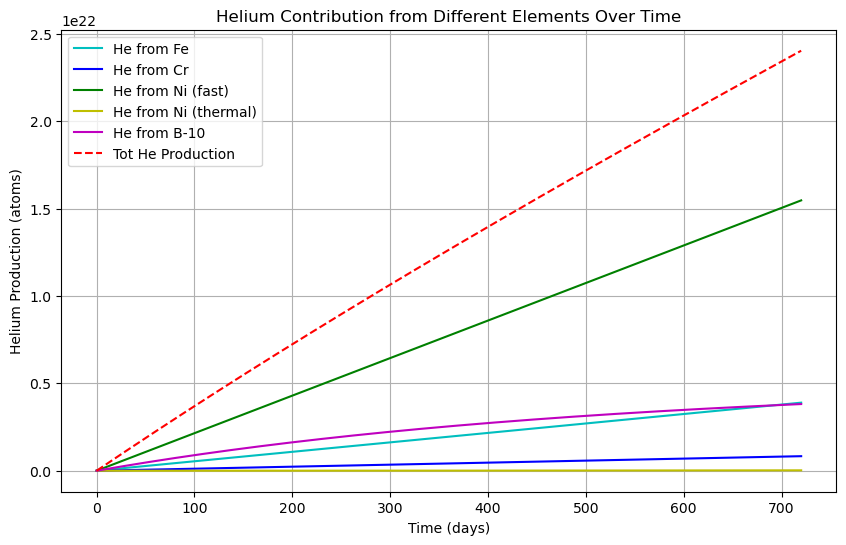
\includegraphics[width=0.6\textwidth]{He_production.png}
    \caption{Helium contribution from different elements over time.}
    \label{fig:helium_production}
\end{figure}

Assuming a conservative model where all helium remains trapped within the cladding material, the helium concentration after 1 year of operation is approximately $67$~ppm, increasing to $122$~ppm after 2 years.  
We should evaluate the ratio between ppm and DPA, this ratio should be less lower then $\sim 10$~ppm/DPA for a fast reactor. For ASI304 steel after 1 year of operation with $20$~DPA (taken as a reference value), 
the ratio is $3.35$~ppm/DPA for one year, which is acceptable. At two years, the ratio is $6.1$~ppm/DPA, which is still below the threshold but might start to cause concerns.
Regardless of the chosen reference value for DPA, the concentration of helium has been verified against those computed by Olander.

\subsubsection{Effects of Helium Embrittlement}

Helium embrittlement arises due to helium accumulation at grain boundaries, leading to:
\begin{itemize}
    \item Reduced ductility and toughness of the cladding.
    \item Increased susceptibility to crack initiation and propagation.
    \item Accelerated creep and swelling under high temperature and irradiation.
\end{itemize}